\documentclass[10pt]{article}

\usepackage{amsmath}                                                                % Math mode $-$ o $$-$$
\usepackage{amssymb}                                                                % Mathematic symbols
\usepackage{mathrsfs}                                                               % Caligraphic letters
\usepackage{amsthm}                                                                 % Theorem-like environments

\usepackage[english]{babel}                                                         % Language (it is important when hyphenating words)
\usepackage[utf8]{inputenc}                                                         % Accented letters and other strange symbols

\usepackage{graphicx}                                                               % Images
\usepackage{float}                                                                  % Puts images where they belong
\usepackage{subcaption}                                                             % Subimages
\usepackage{wrapfig}                                                                % Text and image on the same line
\usepackage{subfiles}                                                               % Subfiles
\usepackage[hidelinks]{hyperref}                                                    % Allows external and internal references
\usepackage[nameinlink]{cleveref}                                                   % Improves internal references
\usepackage[super,square]{natbib}                                                   % Easy bibliography

\usepackage{verbatim}                                                               % Verbatim + multiline comments
\usepackage{anysize}\marginsize{2cm}{2cm}{.5cm}{3cm}                                % Personalizes margins: {L}{R}{U}{D}
\usepackage{bbm}                                                                    % Allows \1
\usepackage{mathdots}                                                               % Rising triple dot symbol
\usepackage{faktor}                                                                 % Fancy rendering of coset sets
\usepackage{tikz-cd}                                                                % Commutative diagrams
\usetikzlibrary{babel}                                                              % Avoids interference between tikz-cd i babel
\usepackage{lipsum}                                                                 % Lorem ipsum dolor sit amet, with \lipsum or \lipsum[1]
\usepackage{todonotes}                                                              % To indicate something is missing
\usepackage[normalem]{ulem}
\usepackage{graphicx}

\usepackage{amsthm}
\usepackage{xcolor}
\usepackage{tcolorbox}
\newtcbox{\mybox}{on line,
  colframe=blue,colback=blue!10!white,
  boxrule=0.5pt,arc=4pt,boxsep=0pt,left=6pt,right=6pt,top=6pt,bottom=6pt}
\usepackage{float}
\usepackage{hyperref}
\hypersetup{
    colorlinks = true,
    filecolor = blue,
    linkcolor = blue,
    urlcolor = blue,
}

\thispagestyle{empty}

\begin{document}
\begingroup
  \centering
  \Huge Wine type and quality determination \\
  \vskip 0.35cm
  \LARGE Intermediate delivery\\
  \vskip 0.25cm
  \large Aleix Torres i Camps, Àlex Batlle Casellas, Luis Sierra Muntané\\[1.5em]
\endgroup


\section{Description and goals of the project.}
Our goal with this project is that of obtaining a data-driven understanding of the relationships between the chemical characteristics of wine and features such as its colour or quality. The data in question is \href{http://archive.ics.uci.edu/ml/datasets/Wine+Quality}{this data set} featuring Portuguese wines of the \textit{Vinho Verde} region and shows 4898 instances of wines of 12 and physiochemical qualities of the wine: 

\begin{ennumerate}
\item fixed acidity
\item volatile acidity
\item citric acid
\item residual sugar
\item chlorides
\item free sulfur dioxide
\item total sulfur dioxide
\item density
\item pH
\item sulphates
\item alcohol
\item quality (score between 0 and 10) - Output variable based on sensory data
\end{ennumerate}

Furthermore, we consider whether the wine is red or white, given that there are two datasets, one for each colour of wine.
\\ As such, the main objective will be that of classifying the wines into their corresponding colour class as white or red from their physiochemical properties, but also to determine their quality on a scale of 1 to 10 as subjectively decided by a panel of experts from their sensory perceptions of the wine. As such, we will want to see whether there are variables which can strongly predict the final quality of a wine or whether such variables are even relevant in determining such a metric. This is especially relevant since the variables, which are all real numbers, are usually associated with being important qualities for the wine and its final taste. It remains to be seen whether they will be good to predict the final factor variables of colour and quality, and to discern which variables yield better models for the prediction of the target variables.

\section{Related previous work.}
This data set has been previously used in various projects, as wine appears to be a frequent topic in examples of classification problems in ML. The first one we cite here is the one provided as a relevant paper, \href{https://www.sciencedirect.com/science/article/pii/S0167923609001377?via\%3Dihub}{Modeling wine preferences by data mining from physicochemical properties}. This paper, as it states in its abstract, proposes a data mining approach to predict human taste preferences on wine, through three different types of regression model: multiple regression, neural networks and support vector machines. This goal is similar to ours, but uses models we cannot comment on for the moment, as they have not been explained in class yet. \\ \ \\
Apart from the data set webpage, we have looked for other projects that cite and use this data set. Searching through Kaggle we have found some different kernels operating on this data. Some of these use decision tree-based methods and support vector machines so we are not commenting on them either. Even though, they also use linear and generalized linear models to preliminary test variable significance. \\ \ \\
The \href{https://www.kaggle.com/indra90/predicting-white-wine-quality}{first kernel} only uses white wine data. One thing to remark about most of the models used on this kernel is that they binarize the quality of the wines into "good" and "not good" and then use the previous stated models and logistic regression. \\ \ \\
In the \href{https://www.kaggle.com/conradws/how-good-is-this-wine-m-l-for-quality-control}{second kernel}, it is remarkable the various ways in which the author tries to gain insight on the data. Initially they use k-Means to cluster data, and then based on the results of this method they visualize the data using a Radial Visualization (RadViz) plot, which we can map into our knowledge as being similar to a biplot. In this way they can observe if there exist any clear tendencies as to variable influence in wine quality. They also pay special attention to anomalies throughout the notebook. \\ \ \\
The \href{https://www.kaggle.com/danielpanizzo/red-and-white-wine-quality}{third kernel} we are commenting on is an exploratory data analysis into the data. In this work it is remarkable the univariate distribution exploration, and especially the fact that this is done separately with white and red wine. This indicates that these two variants might need different treatment, which makes our second task (classification into red or white wine) pertinent in the combined data set. \\ \ \\
We found some additional data exploration notebooks: namely, \href{https://rstudio-pubs-static.s3.amazonaws.com/57835_c4ace81da9dc45438ad0c286bcbb4224.html}{this one} performs some comparative plots between variables and their correlations, and \href{http://rstudio-pubs-static.s3.amazonaws.com/219996_9cc8cf9f2e7e41fe8912454c3ad2685a.html}{this other one} also investigates univariate, bivariate and multivariate relationships between variables.
\section{Data exploration.}
First of all, the data set is given into two different tables, one for red and the other for white wine. Then we decided to perform the union and \textbf{obtain an unique data set}. After that, we extracted the two target vectors. The first one, \textit{wine.type}, determines if the wine is red or white and the second one, \textit{wine.quality}, is the quality value given by the oenologist. \\ \ \\
After some exploration, we detected something that we did not expect: some rows have the exact same values in all of the variables, so we concluded that there are \textbf{duplicated rows} in the data set. So we went back and decided to delete the duplicated ones and leave just one of them. But a major problem was found, 2 rows were at the same time in the two original data sets. In this situation we decided, for now, to delete the rows from both tables, as we do not know whether they belong to red or to white wines, and we still have a lot of other rows. \\ \ \\
Now, we were interested in the \textbf{dimensions of the data set}. So we observed there are 5318 rows and 11 input variables. From these rows, 1357 are red wines and 3959 white. And the table of wine quality with respect to the numbers of rows with that value is:
\begin{table}[H]
\caption{Number of wines of each quality}
\centering
\begin{tabular}{|c|c|c|c|c|c|c|c|}
\hline
wine quality  & 3  & 4   & 5    & 6    & 7    & 8   & 9 \\ \hline
num. of wines & 30 & 206 & 1751 & 2323 & 855  & 148 & 5 \\ \hline
\end{tabular}
\end{table}
\ \\
Then, from these information we may extract some conclusions. The first one is that not all possible marks ([0,10]) were given. And more important, \textbf{the data set is unbalanced} with respect to wine type and wine quality. There are three times white wines as red ones and most of the marks are 6's or 5's, followed by 7's, while the other ones have a very small amount. \\ \ \\
The next thing we did is caring about \textbf{missing values}. After some exploration using \textit{summary} and some \textit{histograms}, the conclusion is that there are no missing values. Although a variable was suspicious, \textit{citric.acid}, because it has a very large amount of 0 values, most of them coming from the white wines. We investigated a little bit on the topic and found that it is a supplement used as a natural preservative or a flavour potential, so we may assume that some wines have no citric acid at all. \\ \ \\
In the review of the data, some \textbf{outliers} were found. Such as some wine with 1.66 in \textit{citric.acid}, while the 3rd quartile of this variable is 0.4, or another with \textit{residual.sugar} 65.8, while its 3rd quartile is 7.5. For the moment we decided to keep them but we may delete them in the future. \\ \ \\
So then, we perform a \textbf{particular analysis of each variable}. We saw that all the variables of the new data set are numerical, therefore we can perform computations over them. But two variables seem to be discrete (\textit{free.sulfur.dioxide} and \textit{total.sulfur.dioxide}). One of the target variables is also discrete and the other is a factor of two elements. \\ \ \\
We start by plotting the \textbf{histograms}, with different colors for each wine type. We detect that for \textit{fixed.acidity}, \textit{volatile.acidity} and \textit{citric.acid}, the two wine types have different behaviours: the white type is more like a normal distribution, while the red is flatter and in some cases looks more like a uniform distribution. These variables have in common that all of them are related to acidity so maybe in the future we might join them and create a unique variable. \\
\begin{figure}[H]
\centering
\caption{Histograms of 3 variables}
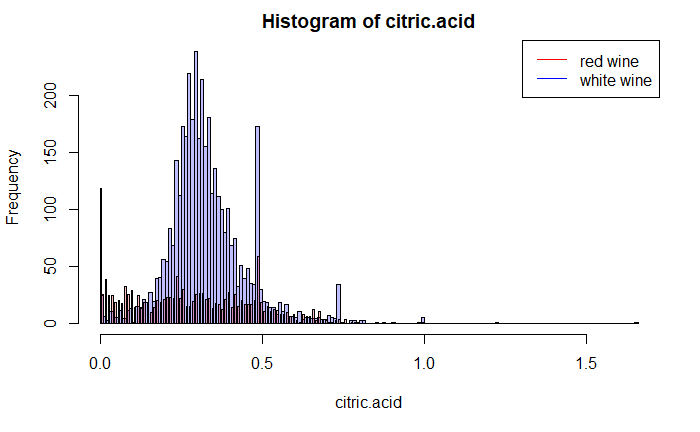
\includegraphics[scale=0.3]{histogram_of_citricacidity}
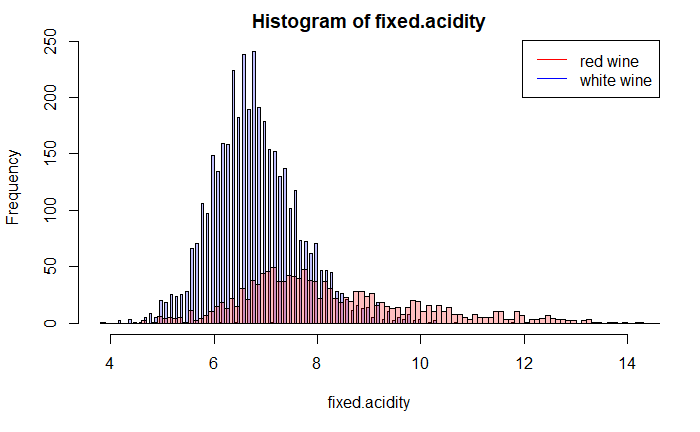
\includegraphics[scale=0.3]{histogram_of_fixedacidity}
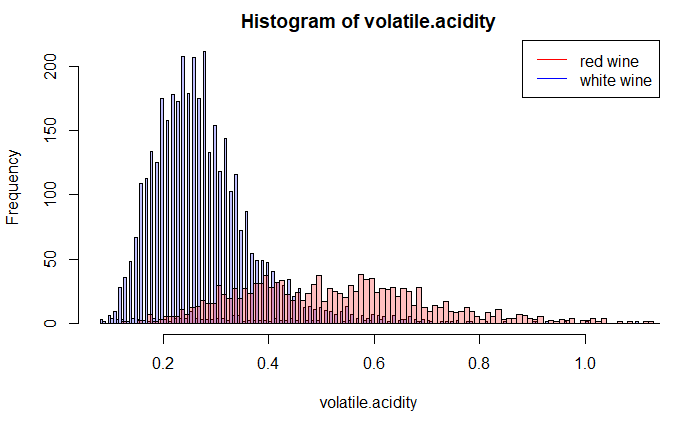
\includegraphics[scale=0.3]{histogram_of_volatileacidity}
\end{figure}
\ \\
The second thing we detected is that the variable \textit{residual.sugar} has a lot of small entries, so we considered applying a logarithm and seeing the result. There is a clear improvement, and something interesting was discovered. The red wine can be modeled as a unique normal distribution while the white wine as two of them, as there are two density regions with a separation between them. So we can treat the logarithm of the \textit{residual.sugar} as a useful \textbf{feature}.
\begin{figure}[H]
\centering
\caption{Histograms of \textit{residual.sugar} and its logarithm}
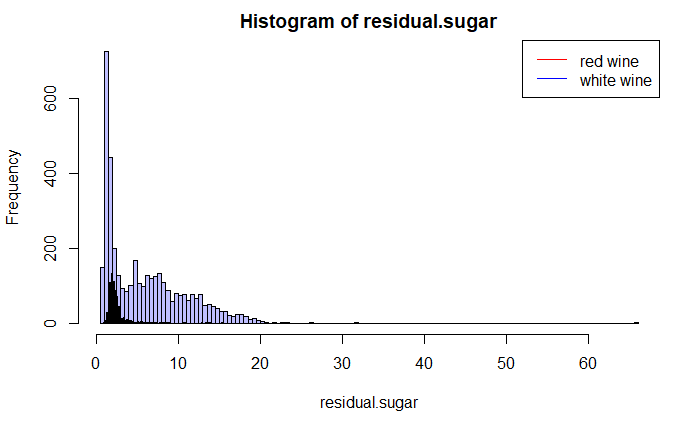
\includegraphics[scale=0.4]{histogram_of_residualsugar}
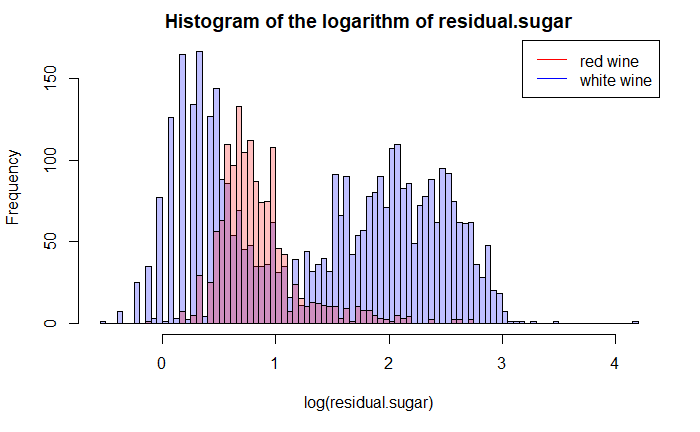
\includegraphics[scale=0.4]{histogram_of_log_residualsugar}
\end{figure}
\ \\
Finally, the other variables' \textit{histograms} have a \textbf{similar shape} in both wine types, but usually with \textbf{different means}. This fact could be useful in order to perform \textit{classification}. And it will be relevant as well for the \textit{regression model} to differentiate the \textit{wine.type} as factors. Here are some of the other \textit{histograms}: \\
\begin{figure}[H]
\centering
\caption{Histograms of 4 variables}
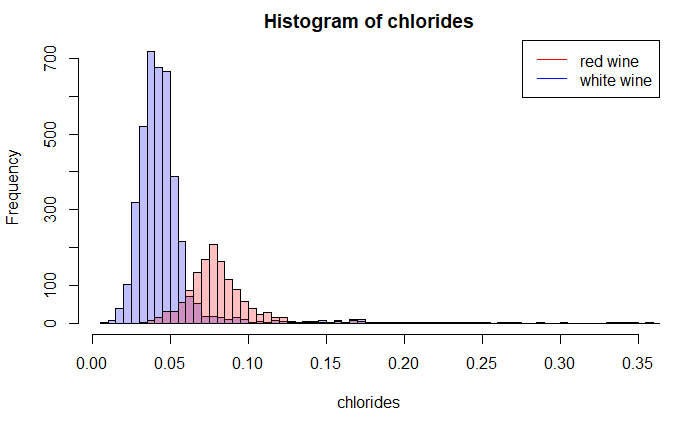
\includegraphics[scale=0.4]{histogram_of_chlorides}
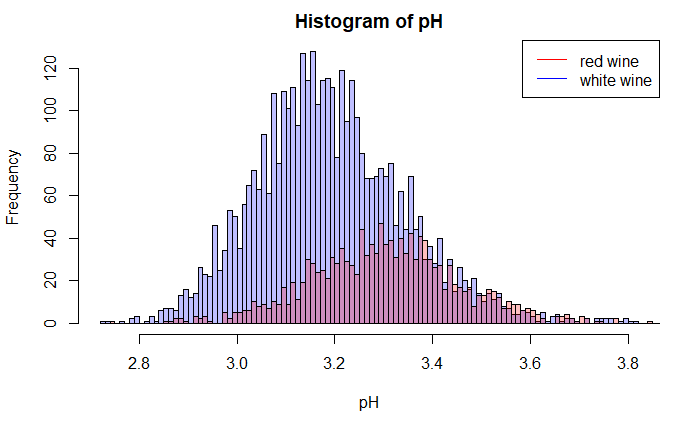
\includegraphics[scale=0.4]{histogram_of_pH}
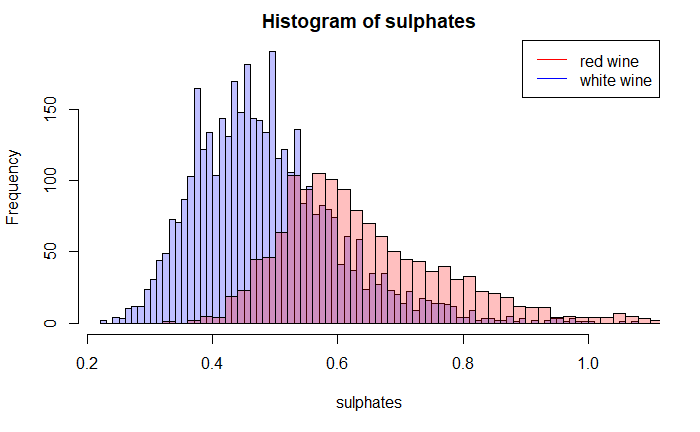
\includegraphics[scale=0.4]{histogram_of_sulphates}
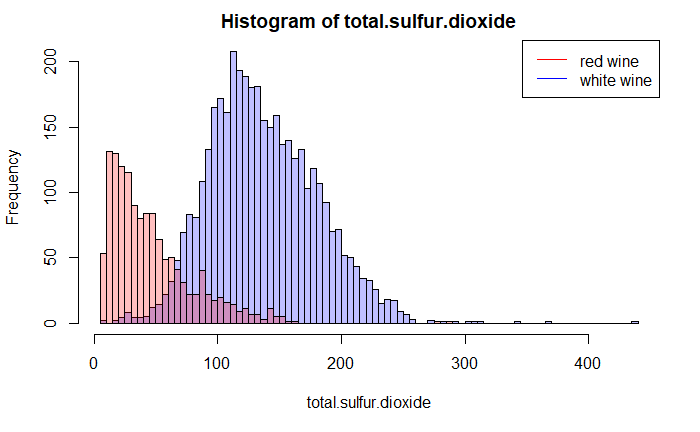
\includegraphics[scale=0.4]{histogram_of_totalsulfurdioxide}
\end{figure}
\ \\
The next thing we considered was performing a \textbf{PCA}, because it can help us visualize the data and start seeing which variables are more relevant to our goal. We made the following \textit{biplot}, where the first two components explain 50\% of the variability. \\
\begin{figure}[H]
\centering
\caption{PCA biplot}
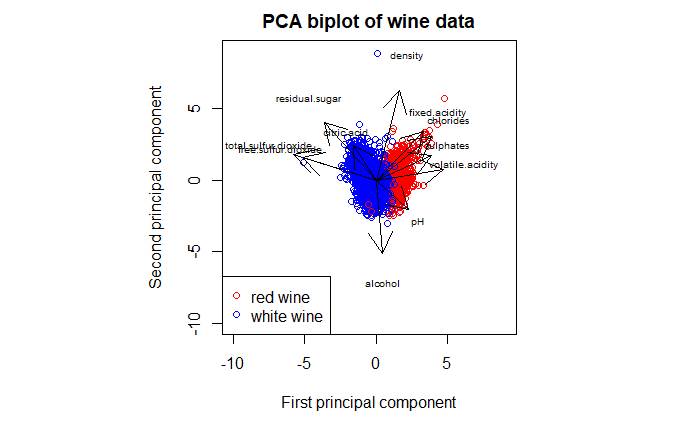
\includegraphics[scale=0.75]{PCA_biplot}
\end{figure}
\ \\
As the two groups seem to be separated in the horizontal edge, it seems that the \textbf{density and alcohol variables explain very little about the difference between the groups}. However, variables such as \textit{total.sulfur.dioxide} or \textit{volatile.acidity} do. In the PCA we can also see that \textbf{some variables are correlated}, for example, \textit{total.sulfur.dioxide} and \textit{free.sulfur.dioxide} in positive or \textit{density} and \textit{alcohol} in negative. There is a last thing to observe here, the \textbf{outliers}. There are points that are not only far from the others on one variable, but they are so in multiple of them. We will consider whether to remove them or not.   \\ \ \\
The next thing we can do is a \textbf{bivariate analysis}. We have already seen that some variables may have correlation among them, thus, it is interesting to do the \textit{correlation matrix}. The following graphic is a representation of it using colored circles. \\
\begin{figure}[H]
\centering
\caption{Correlation matrix}
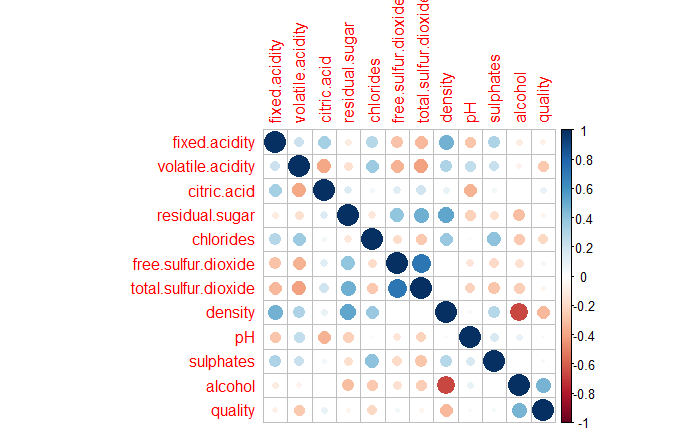
\includegraphics[scale=0.5]{matrix_correlation_circles}
\end{figure}
\ \\
We have added the \textit{quality} variable, as it can help us have an intuition about which input variables could be useful to predict it. As it can be seen, only few of them have a linear correlation with the target variable. Other variables present mutual correlation, as we suspected.

\section{Modeling methods considered.}

\section{Preliminary results.}

\section{Future approaches.}

\section{References:}
\begin{enumerate}
  \item Web page where the data set can be found:

  \href{http://archive.ics.uci.edu/ml/datasets/Wine+Quality}{ http://archive.ics.uci.edu/ml/datasets/Wine+Quality}

  \item Relevant paper (a previous approach):

  \href{https://www.sciencedirect.com/science/article/pii/S0167923609001377?via\%3Dihub}{ https://www.sciencedirect.com/science/article/pii/S0167923609001377?via\%3Dihub}

  \item Kernels that study this data set on Kaggle (\href{www.kaggle.com}{kaggle.com}):

  \href{https://www.kaggle.com/indra90/predicting-white-wine-quality}{First kernel: https://www.kaggle.com/indra90/predicting-white-wine-quality},\\
  \href{https://www.kaggle.com/conradws/how-good-is-this-wine-m-l-for-quality-control}{Second kernel: https://www.kaggle.com/conradws/how-good-is-this-wine-m-l-for-quality-control},\\
  \href{https://www.kaggle.com/danielpanizzo/red-and-white-wine-quality}{Third kernel: https://www.kaggle.com/danielpanizzo/red-and-white-wine-quality}.

  \item Exploratory Data Analysis notebooks:

  \href{https://rstudio-pubs-static.s3.amazonaws.com/57835\_c4ace81da9dc45438ad0c286bcbb4224.html}{ https://rstudio-pubs-static.s3.amazonaws.com/57835\_c4ace81da9dc45438ad0c286bcbb4224.html},\\
  \href{https://rstudio-pubs-static.s3.amazonaws.com/219996\_9cc8cf9f2e7e41fe8912454c3ad2685a.html}{ https://rstudio-pubs-static.s3.amazonaws.com/219996\_9cc8cf9f2e7e41fe8912454c3ad2685a.html}.



\end{enumerate}



\end{document} 